% Local CVPR 2027 draft based on a pinned PROVISIONAL_2026 kit.
% This is a scaffold, not an official 2027 template or a submission-ready paper.
\documentclass[10pt,twocolumn,letterpaper]{article}
% T1 selects the official Times font metrics with XeTeX/Tectonic as well as pdfLaTeX.
\usepackage[T1]{fontenc}
\usepackage[review]{cvpr}
% Project additions; no margin, font-size, or spacing overrides.
\usepackage{amsmath,amssymb}
\usepackage{booktabs}
\usepackage{tabularx}
\usepackage{xcolor}
\usepackage{tikz}
\usetikzlibrary{positioning,arrows.meta,fit,calc,backgrounds}
\usepackage{algorithm}
\usepackage{algpseudocode}
\newif\ifhasverifiedreferences
\hasverifiedreferencestrue % Draft 1: 19 entries; each copied from a local PDF or a publisher page.
\newcommand{\draftnote}[1]{\par\noindent\textbf{Draft status:} #1\par}
\newcommand{\notmeasured}{\textit{n/m}}
% Pending content is shown in red and must be resolved or removed before submission.
\newcommand{\tbd}[1]{{\color{red}[TBD: #1]}}
% Numbers traceable to a verify.json / summary.json but not yet in paper/evidence registry: dark orange in draft.
% Redefine as identity (\renewcommand{\pend}[1]{#1}) once the registry audit passes.
\newcommand{\pend}[1]{{\color{orange!75!black}#1}}
\newcommand{\sys}{AG3S}% method name as in the working title
\newcommand{\dmain}{d}
\newcommand{\dfree}{d^{\star}}

\definecolor{cvprblue}{rgb}{0.21,0.49,0.74}
\usepackage[pagebackref,breaklinks,colorlinks,allcolors=cvprblue]{hyperref}
% Working metadata, separate from the immutable official kit.
\def\paperID{*****} % Replace with the actual registered OpenReview paper ID.
\def\confName{CVPR}
\def\confYear{2027} % Local target year; does NOT make this a 2027 official kit.
\title{AG3S VLA: Grounding VLA Attention in 3D\\for Task-Dependent Contact Constraints}% revised working title; subject to final results
\author{Anonymous Authors}

\begin{document}
\maketitle
\begin{center}
\textbf{DRAFT --- EVIDENCE PENDING}\\
Provisional 2026 style; working target: CVPR 2027.
\end{center}
% !TEX root = ../main.tex
\begin{abstract}
Geometric collision avoidance for vision-language-action (VLA) policies must distinguish necessary object contact
from unwanted collision. This requires identifying the task target, recovering its spatial extent, and determining
which robot links may contact it as manipulation proceeds. We present \sys, which connects a frozen VLA's internal
visual signals to task-dependent geometric constraints. Action-to-image attention seeds multi-view 3D clustering,
providing target geometry without an external detector or segmentation network. This geometry defines a local
contact exception for selected gripper links, while other modeled links query a scene distance field containing
the target. A lightweight probe trained on frozen features controls target-identity updates across manipulation
phases, and a grasp state machine transfers grasped geometry into attached-object collision queries. The resulting
constraints refine the executed portion of each action chunk. The VLA requires no additional training for collision
avoidance. \tbd{Insert verified task success, forbidden-contact and safe-success results, plus the key
matched-controller ablation demonstrating the contribution of target geometry and link-specific contact handling.}
\end{abstract}

% !TEX root = ../main.tex
% Draft 10: claim/source map in notes/DRAFT10_REVISION.md. Performance claims remain pending.
\section{Introduction}
\label{sec:introduction}
% Native vector schematic; no synthetic or illustrative performance data.
\begin{minipage}{\textwidth}
\centering
\captionsetup{type=figure,hypcap=false}
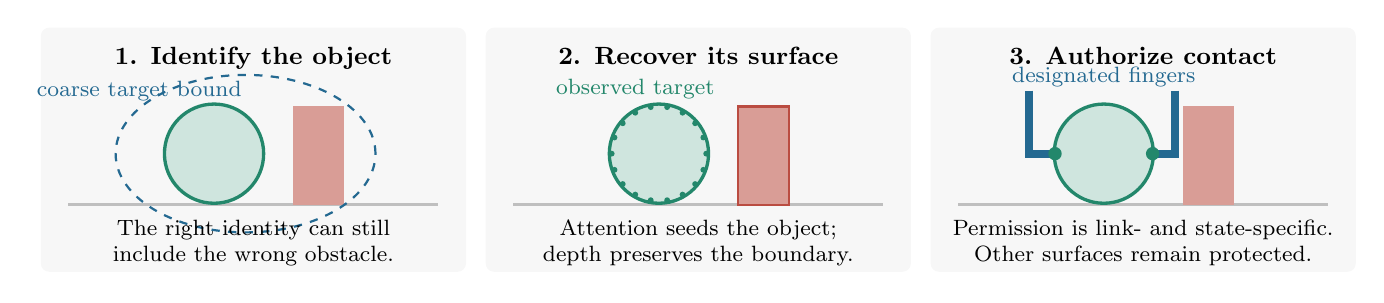
\begin{tikzpicture}[x=1cm,y=1cm,>=Latex,font=\small]
\definecolor{targetgreen}{RGB}{35,135,107}
\definecolor{protectred}{RGB}{186,76,65}
\definecolor{policyblue}{RGB}{36,105,145}
\foreach \x/\title in {0/1. Identify the object,5.65/2. Recover its surface,11.3/3. Authorize contact}{
 \fill[black!3,rounded corners=3pt] (\x,0) rectangle +(5.4,3.1);
 \node[anchor=north,font=\small\bfseries] at (\x+2.7,2.98) {\title};
 \draw[black!25,line width=1pt] (\x+.35,.85)--(\x+5.05,.85);
 \fill[targetgreen!22] (\x+2.2,1.5) circle (.63);
 \draw[targetgreen,line width=1.2pt] (\x+2.2,1.5) circle (.63);
 \fill[protectred!55] (\x+3.2,.85) rectangle +(0.65,1.25);
}
\draw[policyblue,dashed,thick] (2.6,1.5) ellipse (1.65 and 1.0);
\node[policyblue,font=\footnotesize] at (1.25,2.3) {coarse target bound};
\node[align=center,font=\footnotesize] at (2.7,.37) {The right identity can still\\include the wrong obstacle.};
\foreach \a in {0,20,...,340}{
 \fill[targetgreen] ({7.85+.60*cos(\a)},{1.5+.60*sin(\a)}) circle (.037);
}
\draw[protectred,thick] (8.85,.85) rectangle +(0.65,1.25);
\node[targetgreen,font=\footnotesize] at (7.55,2.32) {observed target};
\node[align=center,font=\footnotesize] at (8.35,.37) {Attention seeds the object;\\depth preserves the boundary.};
\draw[policyblue,line width=3pt] (12.55,2.3)--(12.55,1.5)--(12.85,1.5);
\draw[policyblue,line width=3pt] (14.4,2.3)--(14.4,1.5)--(14.15,1.5);
\fill[targetgreen] (12.88,1.5) circle (.085);
\fill[targetgreen] (14.12,1.5) circle (.085);
\node[policyblue,font=\footnotesize] at (13.5,2.48) {designated fingers};
\node[align=center,font=\footnotesize] at (14,.37) {Permission is link- and state-specific.\\Other surfaces remain protected.};
\end{tikzpicture}
\caption{\textbf{Identity, extent, and permission are different decisions.}
\sys\ uses internal noun attention to seed an observed 3D surface graph. The selected surface defines the intended extent of a contact exception; a coarse bound does not. The final panel illustrates link-specific contact permission; after grasping, the target becomes attached geometry checked against the environment. All panels illustrate the proposed mechanism, not measured execution outcomes.}
\label{fig:teaser}
\end{minipage}


A robot reaching for an apple must distinguish two geometrically similar events: its fingers touching the apple and its
wrist striking a nearby object. The distinction depends on the instruction, the robot link, and the stage of manipulation.
After grasping, the apple itself becomes moving geometry that must clear the environment; after release, it becomes part
of the scene again. This changing role of the same visible surface is a central difficulty in connecting
vision-language-action (VLA) policies to geometric collision avoidance.

VLAs such as $\pi_0$, $\pi_{0.5}$, and GR00T N1 generate action chunks from visual observations and language
instructions~\cite{black2024pi0,intelligence2025pi05,nvidia2025gr00t}. Their task-conditioned behavior makes them a useful
source of manipulation proposals, but successful task completion alone does not establish collision-free
execution~\cite{fan2026safevlabench}. Depth-based distance fields provide an explicit account of surrounding surfaces
for motion generation~\cite{sundaralingam2023curobo,sundaralingam2026curobov2}. Geometry alone, however, does not specify
which of those surfaces a particular link may touch. Treating the target as an obstacle can prevent the grasp; removing
it from a shared collision field also removes it for links that should still avoid it. The missing connection is from
\emph{visual task relevance} to \emph{spatially and temporally selective contact constraints}.

Prior work provides several parts of this connection. VLSA uses external visual grounding to configure a safety
filter~\cite{hu2026vlsa}, and MoManipVLA excludes a segmented target from its distance-field reconstruction in its
real-world pipeline~\cite{wu2025momanipvla}. KNOWS uses VLA attention to select a target among objects supplied by a
segmentation model~\cite{park2026knows}. Thus, attention-based target selection and target exclusion are established
ideas. What remains to be addressed here is how to recover the target's spatial extent directly from VLA signals and
depth, and use that geometry to determine contact permissions for individual links as manipulation proceeds.

Our approach separates the roles of attention and geometry: \emph{attention selects a candidate object, while depth
defines its observed extent}. We present \sys, which grounds action-to-image attention in a multi-view point cloud
without an external detector or segmentation network. Attention seeds geometric clustering rather than masking the
collision map, so weakly attended surfaces remain available as obstacles. The selected target then defines a local
contact exception for the active hand. Other modeled links continue to query the scene field containing the target.
When a grasp is confirmed, the target is represented as geometry attached to the hand and checked against the
environment. This couples object grounding to the geometric consequences of interaction (Fig.~\ref{fig:overview}).

To control when target identities may change and when an exception should end, we also train a lightweight linear
sub-task probe on frozen VLA features. Its predictions supplement a grasp state machine driven by execution feedback;
the state machine determines attachment and detachment. An optimization layer uses the resulting constraints to
refine the portion of each action chunk that will be executed. The VLA remains frozen after embodiment fine-tuning:
\emph{no additional VLA training for collision avoidance is required}. The probe is trained separately, and the current
implementation reads attention through an additional pass of the same checkpoint.

The contribution is the connection from internally derived target geometry to phase- and link-specific constraints.
We develop it through:
\begin{itemize}
\item An attention-to-geometry procedure that extracts an observed 3D target from a frozen VLA and calibrated depth,
without an external segmentation model or a separately supplied target name.
\item A contact representation that uses this target geometry for link-specific distance queries, manages its lifetime
with sub-task and grasp-state information, and transfers grasped geometry to the robot's collision queries.
\item \tbd{A controlled evaluation: insert verified task success, forbidden-contact and safe-success results, then state
what target grounding and link-specific handling add under the same refinement controller.}
\end{itemize}
The evaluation separates target identity, geometric extent, and contact handling so that improved execution can be
attributed to the information supplied to the controller rather than to a change of controller alone.

% !TEX root = ../main.tex
% Scoped primary-source checks and remaining verification: notes/DRAFT10_REVISION.md.
\section{Related Work}
\label{sec:related}

\paragraph{VLA policies and geometric action refinement.}
Flow-based VLAs generate action chunks conditioned on visual and language features~\cite{black2024pi0,intelligence2025pi05,nvidia2025gr00t}.
Their outputs can serve as references for geometric optimization. MoManipVLA transfers VLA-generated end-effector
trajectories to mobile manipulation through optimization with scene geometry~\cite{wu2025momanipvla}. More generally,
cuRobo and cuRoboV2 provide GPU-accelerated motion generation, including collision queries and depth-fused distance
fields~\cite{sundaralingam2023curobo,sundaralingam2026curobov2}. These works motivate our use of a frozen policy and a
geometric refinement layer. Our focus is the information supplied to that layer: how a visually identified target
changes the collision constraints of particular robot links.

\paragraph{Grounding from internal visual representations.}
Selected attention heads in frozen vision-language models can localize referred objects~\cite{kang2025fewheads}.
KNOWS brings this idea to manipulation by using VLA attention to rank objects produced by a fine-tuned YOLOE
segmenter, then applying an ellipsoid-based safety filter~\cite{park2026knows}. It is the closest precedent for using
internal attention to select a contact target. Our target geometry is instead constructed by lifting attention into
depth and growing regions in the observed 3D cloud. This avoids requiring a segmentation model to enumerate candidate
objects and supplies a geometric region for link-specific distance queries. Attention is used as a selection cue;
the quality of the resulting extent must be assessed separately from target identity.

\paragraph{Task-dependent collision geometry.}
VLSA uses a vision-language model and visual grounding to identify obstacles for action
filtering~\cite{hu2026vlsa}. Lan-o3dp combines language-guided object decomposition and segmentation with
collision-aware diffusion-policy execution~\cite{li2025lano3dp}. MoManipVLA's real-world pipeline excludes the target
mask from ESDF construction~\cite{wu2025momanipvla}. Stage-dependent geometry is also used in AutoMoMa, which generates
whole-body trajectories in known scenes and incorporates manipulated objects into the robot's kinematic
representation~\cite{niu2026automoma}. WBAG explicitly models whole-body and grasp-dependent attached geometry for
VLA filtering~\cite{zhen2026wbag}. We build on the need for such contact-dependent representations. Our distinction is
to construct the contact target from VLA attention and observed depth, retain separate distance queries for contact
and non-contact links, and manage these queries during chunk refinement. The current robot query model covers
gripper links and attached-object approximations; it does not provide whole-body coverage.

\paragraph{Reading task state from frozen policies.}
$\pi_{0.5}$ and LoHoVLA incorporate sub-task prediction into their learned policy
structure~\cite{intelligence2025pi05,yang2025lohovla}. Probing studies also recover task progress and success-related
signals from frozen VLA representations~\cite{bhardwaj2026progress,zhang2026frozenvlas}. We use a supervised linear probe
for three manipulation phases and apply its output to target adoption and exception termination. The probe supports
the contact representation; it neither modifies the VLA weights nor generates the policy's action sequence.
Its value beyond a grasp-state rule is an empirical question addressed by a matched-controller comparison.

% !TEX root = ../main.tex
% Draft 10 describes the V7g design and checked source interfaces, not registered experimental performance.
% Source pointers and final-configuration TBDs: notes/DRAFT10_REVISION.md.
\section{Method}
\label{sec:method}
\sys\ connects visual target grounding to contact-aware action refinement. Attention-based Target Segmentation (ATS)
extracts target geometry; a Hidden-state Sub-task Recognition (HSR) probe helps maintain its identity across phases;
Link-specific Target Exemption (LTE) converts it into distance queries for individual links. Constrained Chunk
Refinement (CCR) applies those queries to the executed action horizon. Figure~\ref{fig:overview} summarizes the data flow.

% F02: Draft 10 conceptual data flow; separate serving and extraction passes are explicit.
\begin{figure*}[t]
\centering
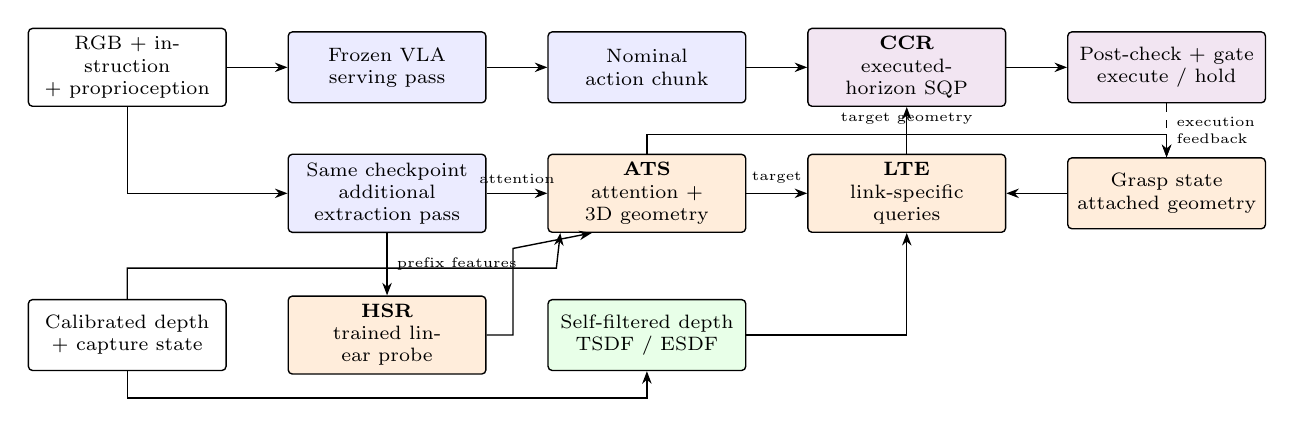
\begin{tikzpicture}[
  x=1cm,y=1cm,font=\scriptsize,>={Stealth[length=1.6mm]},
  box/.style={draw,rounded corners=1.5pt,align=center,inner sep=3pt,text width=23mm,minimum height=9mm},
  pol/.style={box,fill=blue!8}, geo/.style={box,fill=green!9},
  tgt/.style={box,fill=orange!14}, opt/.style={box,fill=violet!10},
  every path/.style={line width=0.5pt}]
\node[box] (obs) at (0,3) {RGB + instruction\\+ proprioception};
\node[pol] (pi) at (3.3,3) {Frozen VLA\\serving pass};
\node[pol] (chunk) at (6.6,3) {Nominal\\action chunk};
\node[opt] (sqp) at (9.9,3) {\textbf{CCR}\\executed-horizon SQP};
\node[opt] (gate) at (13.2,3) {Post-check + gate\\execute / hold};
\node[pol] (extract) at (3.3,1.4) {Same checkpoint\\additional extraction pass};
\node[tgt] (ats) at (6.6,1.4) {\textbf{ATS}\\attention + 3D geometry};
\node[tgt] (lte) at (9.9,1.4) {\textbf{LTE}\\link-specific queries};
\node[tgt] (grasp) at (13.2,1.4) {Grasp state\\attached geometry};
\node[box] (depth) at (0,-0.4) {Calibrated depth\\+ capture state};
\node[tgt] (hsr) at (3.3,-0.4) {\textbf{HSR}\\trained linear probe};
\node[geo] (field) at (6.6,-0.4) {Self-filtered depth\\TSDF / ESDF};
\draw[->] (obs)--(pi); \draw[->] (pi)--(chunk); \draw[->] (chunk)--(sqp); \draw[->] (sqp)--(gate);
\draw[->] (obs.south) |- (extract.west);
\draw[->] (extract)--node[above,font=\tiny]{attention}(ats);
\draw[->] (extract)--node[right,font=\tiny]{prefix features}(hsr);
\draw[->] (hsr.east)--(4.9,-0.4)--(4.9,0.7)--([xshift=-7mm]ats.south);
\draw[->] (ats)--node[above,font=\tiny]{target}(lte);
\draw[->] (ats.north)--(6.6,2.15)--node[above,font=\tiny]{target geometry}(13.2,2.15)--(grasp.north);
\draw[->] (depth.south)--(0,-1.2)--(6.6,-1.2)--(field.south);
\draw[->] (depth.north)--(0,0.45)--(5.45,0.45)--([xshift=-11mm]ats.south);
\draw[->] (field.east)-|(lte.south);
\draw[->] (lte)--(sqp);
\draw[->] (grasp)--(lte);
\draw[->,dashed] (gate)--node[right,font=\tiny,align=left]{execution\\feedback}(grasp);
\end{tikzpicture}
\caption{\textbf{System overview.} The VLA serving pass produces the nominal chunk. A separate pass of the same frozen
checkpoint supplies attention for ATS and cached features for the trained HSR probe. Target geometry, phase-dependent
identity updates, and grasp state configure the link-specific queries used by CCR. Dashed feedback denotes recorded
execution information. The diagram describes the method, not measured performance.}
\label{fig:overview}
\end{figure*}


\subsection{Task-conditioned geometric constraints}
\label{sec:overview}
At request $t$, a frozen VLA receives RGB images, proprioception, and an instruction $l$, denoted by $(o_t,l)$, and
predicts an action chunk $A_t=\pi_\theta(o_t,l)$. Only its first $K$ of $H$ rows will be executed before replanning.
We refine the arm-joint references $Q^{\mathrm{ref}}\in\mathbb{R}^{K\times n_q}$ in those rows; gripper commands and
the remaining rows are passed through unchanged. Calibrated depth is an additional input to the geometric layer.
The active manipulator and its contact-link set $\mathcal L$ are supplied to the system.

Let $\mathcal T_t$ denote the observed target geometry, $s_t$ the inferred sub-task, and $z_t$ the grasp state.
Together they determine a distance query $\delta_{i,t}$ for each modeled robot or attached-object sphere $i$.
For center $c_i(q_k)$, radius $r_i$, and margin $m_{ik}$, we define
\begin{equation}
h_{ik}(Q)=\delta_{i,t}\big(c_i(q_k)\big)-r_i-m_{ik}.
\label{eq:clearance}
\end{equation}
Refinement seeks a trajectory close to the VLA reference while satisfying these modeled clearance constraints and
joint limits. The key dependence is in $\delta_{i,t}$: the same surface can be permitted for a contact link, retained
for another link, or represented as an attached object. Sections~\ref{sec:grounding}--\ref{sec:exemption} construct this
dependence; Sec.~\ref{sec:refine} describes the optimizer.

\subsection{From VLA attention to target geometry}
\label{sec:grounding}
An attention peak indicates a candidate location, but does not provide the object's full 3D extent. Conversely,
geometric clustering separates spatial regions without identifying which one the policy is manipulating. ATS combines
these signals by using attention to seed and rank geometric regions (Fig.~\ref{fig:fig03_attention_to_3d}).

\paragraph{Attention and multi-view lifting.}
For each camera $v$, we read an action-to-image attention map $\alpha_t^v$ from a fixed layer and head at the first
denoising step. The current implementation uses layer~8, head~2, and the last action-token query, producing a
$16\times16$ map for each of three views. An instrumented copy of the same frozen checkpoint performs an additional
prefix and first-denoising-step pass; it is separate from the pass serving actions. HSR reuses the prefix cache of
this extraction pass. \tbd{Document the attention-head selection data and its separation from final evaluation.}

We upsample $\alpha_t^v$ into the depth image coordinates. A valid pixel $u$ with depth $D_t^v(u)$ is lifted by
\begin{equation}
x_t^v(u)=T_t^v\!\left[D_t^v(u)(K^v)^{-1}\widetilde u\right],
\label{eq:lift}
\end{equation}
where $K^v$ is the camera intrinsic matrix and $T_t^v$ maps camera coordinates to the robot base at capture time.
Robot observations are self-filtered. The resulting points are fused on a voxel grid, retaining the maximum
attention value of observations within each voxel and then rescaling the fused attention by percentiles.
Low attention does not remove geometry from the scene map.

\paragraph{Geometric extent and target selection.}
We fit support planes and take high-attention, non-support points as seeds. Density-based clustering~\cite{ester1996dbscan}
grows candidate regions using the full non-support cloud, including low-attention points. Candidates are ranked by
their mean attention, compactness, and proximity to the attention peak. We filter candidates using gripper aperture,
support height, and a persistent destination estimate. In the current pick-and-place implementation, a persistent
high-ranked non-graspable cluster supplies the destination estimate. This is a geometric heuristic, not a general
semantic recognizer of receptacles.

The selected cluster supplies $\mathcal T_t$. A competing identity must persist across requests before replacing it;
during grasp approach and closure, switching additionally requires evidence that the old target is lost and the hand
has moved away. We retain the pre-closing geometry during closure to reduce shrinkage from finger occlusion. This
geometry is an estimate of the observed object, not a completed model of its unseen surface. A geometrically merged
target and obstacle can therefore produce an incorrect exemption; the evaluation must measure extent quality as
well as identity accuracy.

\begin{figure*}[t]
\centering
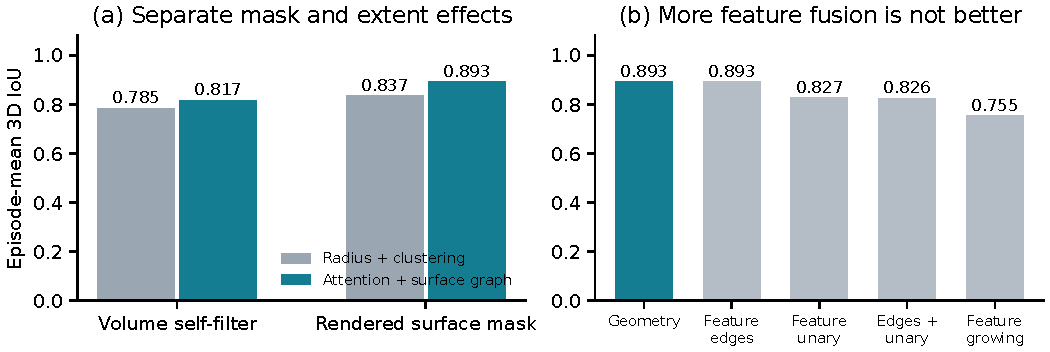
\includegraphics[width=\textwidth]{../figures/ifg_results/results.pdf}
\caption{\textbf{Measured development evidence.}
(a) The rendered robot mask improves both methods; the proposed extent pipeline retains an advantage when the mask is matched.
(b) With that improved geometry fixed, prefix-layer-8 feature edges leave IoU nearly unchanged, while prototype unaries and feature-conditioned growing reduce it.
All bars show episode-mean observed-surface IoU over 32 development episodes; they do not report held-out segmentation or physical safety.}
\label{fig:fig03_attention_to_3d}
\end{figure*}


\subsection{Maintaining the target across manipulation phases}
\label{sec:phase}
Target identity and physical attachment require different signals. HSR supplies a coarse phase for controlling
identity updates; a grasp state machine uses executed gripper commands, measured opening, and geometric evidence to
determine attachment and detachment.

\paragraph{A trained probe on frozen features.}
Let $\mathcal V_t$ be the value vectors at layer~4, key-value head~0 of the extraction pass. We concatenate means over
valid text tokens and image tokens into a feature $f_t\in\mathbb R^{512}$ and predict
\begin{equation}
p_t=\operatorname{softmax}\!\left(W\frac{f_t-\mu}{\sigma}+b\right).
\label{eq:probe}
\end{equation}
The normalization and linear classifier are fitted using phase annotations from the embodiment demonstrations,
with VLA weights held fixed. Text-token features include the instruction and tokenized state. The three classes are
\emph{pick}, \emph{place}, and \emph{home}; \emph{home} denotes post-release retreat and return. The predicted label is
confirmed over three consecutive requests. This is supervised probe training, not additional VLA training for
collision avoidance. \tbd{Finalize the probe training/validation split and phase-label specification in Appendix C.}

\paragraph{Phase and grasp-state roles.}
The confirmed phase controls target adoption and switching as in Table~\ref{tab:subtask}. It does not directly turn an
object into attached geometry. A retained target may still allow grasp contact while the phase has already changed
to \emph{place} but the grasp is unconfirmed. Once the grasp state is \textsc{held}, the representation changes as
described below. Release or detected slip detaches the object; a subsequent confirmed \emph{home} label clears the
retained target identity after \textsc{placed} has been observed. This distinction prevents phase predictions from
being treated as physical grasp measurements.

\begin{table}[t]
\centering\small
\begin{tabularx}{\columnwidth}{@{}l>{\raggedright\arraybackslash}X@{}}
\toprule
Confirmed phase & Target-identity rule \\
\midrule
\emph{pick} & Permit candidate adoption and persistent switching. \\
\emph{place} & Block new adoption and switching; retain the current identity. \\
\emph{home} & Block adoption/switching; clear the identity after \textsc{placed}. \\
\bottomrule
\end{tabularx}
\caption{HSR gates target identity. Before a label is confirmed, the underlying geometric selection rules apply.
Attachment and detachment are controlled separately by the grasp state.}
\label{tab:subtask}
\end{table}

\subsection{Link-specific contact and attached geometry}
\label{sec:exemption}
\paragraph{Scene distance field.}
Self-filtered depth is integrated into a TSDF and converted to an ESDF with the cuRobo mapper~\cite{sundaralingam2026curobov2}.
The scene distance $d_t$ combines coarse coverage with a finer window around the hand's swept region. The target
remains in this scene field before attachment. Unobserved space is treated as free by the current implementation;
therefore the constraints concern reconstructed surfaces.

\paragraph{A separate query for contact links.}
When a target is retained and no object is attached, LTE constructs a second fine ESDF by removing seed voxels in a
ball fitted to $\mathcal T_t$, padded by one voxel and clipped above the support plane. This does not alter the scene
field queried by other links. Let $f_t(x)$ be the target-excluded fine field, $\mathcal W_t$ its spatial window, and
$b_t(x)$ the distance to that window's boundary. The implemented query is
\begin{equation}
\dfree_t(x)=
\begin{cases}
\min\{f_t(x),\max\{d_t(x),b_t(x)\}\}, & x\in\mathcal W_t,\\
d_t(x), & \text{otherwise}.
\end{cases}
\label{eq:exempt}
\end{equation}
The boundary term accounts for the limited extent of the fine field. Defining $e_t=1$ when this exception is active,
the robot-link queries are
\begin{equation}
\delta_{i,t}(x)=
\begin{cases}
\dfree_t(x), & i\in\mathcal L\ \text{and}\ e_t=1,\\
d_t(x), & \text{otherwise}.
\end{cases}
\label{eq:linkquery}
\end{equation}
Here $\mathcal L$ contains the palm and fingers of the supplied active hand. Thus the exception is specific to a
geometric region and a link set. Because the removed region approximates the target with a ball, nearby surfaces
inside that region may also be removed from the contact-link field. The unmodified scene field remains available
to non-contact links; selectivity within the excluded region depends on target geometry quality.

\paragraph{From scene object to attached object.}
On a confirmed grasp, pre-closing target points are transformed into the palm frame and approximated by attached
query spheres. The observed body estimate is used to limit sphere size and offset. Its volume is cleared from the
environment map to avoid counting the object as an obstacle to itself, and its moving spheres query the remaining
environment with a destination clearance term. Attachment therefore changes both sides of the collision query:
the object leaves the environment representation and joins the moving geometry. After detachment, subsequent depth
observations reintroduce it into the scene. The fitted spheres approximate observed extent; coverage of the true
object must be checked for the shapes used in evaluation.

\subsection{Refining and checking the executed chunk}
\label{sec:refine}
CCR uses sequential quadratic programming (SQP) over the executed horizon. Its trajectory objective is
\begin{equation}
\begin{aligned}
J(Q)={}&w_{\mathrm t}\|Q-Q^{\mathrm{ref}}\|_F^2
       +w_{\mathrm s}\|\Delta^2Q\|_F^2\\
      &+w_{\mathrm c}\|Q_{\mathcal O}-\bar Q^{\mathrm{prev}}_{\mathcal O}\|_F^2,
\end{aligned}
\label{eq:qp}
\end{equation}
where $\mathcal O$ is the available overlap with the previous chunk shifted according to execution feedback.
With execution feedback enabled, invalid or unexecuted history is omitted. At iterate $Q^j$, clearance constraints are
linearized as
\begin{equation}
h_{ik}(Q^j)+\langle\nabla h_{ik}(Q^j),Q-Q^j\rangle_F+\xi_{ik}\ge\beta,
\label{eq:linearized}
\end{equation}
where $\langle\cdot,\cdot\rangle_F$ is the Frobenius inner product and $\beta$ is a clearance buffer, with nonnegative
slack $\xi$ penalized by $w_{\xi}\|\xi\|_1$. Each QP includes joint-position bounds, softened velocity
and acceleration bounds, and a trust region, and is solved with OSQP~\cite{stellato2020osqp}. A subset of low-clearance
rows enters the QP; the candidate is subsequently checked against all configured rows at the command waypoints.
Slack-assisted optimization does not itself establish feasibility.

\paragraph{Execution gate.}
The execution gate combines the post-check, field validity, and solver status. A rejected chunk holds the arm at
its measured pose while preserving the gripper command. The current implementation also has a collision-only
fallback: a refined chunk may be accepted when modeled spheres are nonpenetrating and its minimum clearance is no
worse than at the current pose, even if a positive margin is unmet. \tbd{Freeze the final gate configuration and report
fallback use separately in Appendix D.} These checks apply to the configured query geometry and sampled waypoints;
they are not a continuous-time or whole-body safety guarantee.

\paragraph{Implementation scope.}
We instantiate the layer with an embodiment-fine-tuned $\pi_{0.5}$, two 7-DoF arms, and two gripper channels
($H=50$, $K=8$). The client executes commands at 15\,Hz, giving a nominal chunk duration of 533\,ms; this is a timing
budget, not a measured system latency. The present collision queries cover gripper links and attached-object
approximations, with self-collision disabled. ATS thresholds, field resolutions, query geometry, probe fitting, and
solver settings belong in the implementation appendix. \tbd{Finalize the experiment snapshot and Appendix B--D
settings; measure the complete policy, extraction, geometry, refinement, and communication cost.}

% !TEX root = ../main.tex
% Draft 10: evaluation skeleton aligned to the revised claim; no new experiment has been run.
\section{Experiments}
\label{sec:experiments}
The evaluation is organized around five questions:
\textbf{Q1}, how task completion and forbidden contact change;
\textbf{Q2}, what attention contributes to target identity and geometric extent;
\textbf{Q3}, what phase information adds beyond grasp-state rules;
\textbf{Q4}, which contact representation matters under a fixed controller; and
\textbf{Q5}, what the complete system costs at run time.
\tbd{Finalize the evaluation protocol and replace this skeleton with registered results.}

\subsection{Experimental setup}
\paragraph{Tasks and policy.}
The existing implementation uses a $\pi_{0.5}$ checkpoint fine-tuned for dual-arm pick-and-place in MuJoCo~\cite{todorov2012mujoco},
with one supplied active manipulator per episode. The diagnostic scenes place distractors near the grasp target and
obstacles along the carrying path. Simulation uses rendered depth and waits for the inference server.
\tbd{Fix the evaluated snapshot, scene conditions, episodes, seeds, and training/tuning/test separation.}
SafeLIBERO~\cite{hu2026vlsa} is the planned primary benchmark, while the RB-Y1 simulation supports baseline comparisons
and component ablations. A real RB-Y1 demonstration is planned to assess execution feasibility, without a comparative
performance claim. \tbd{Complete the SafeLIBERO observation/action adapter, fix its checkpoint and evaluation suites,
and document whether phase handling uses HSR or a grasp-state rule. Keep robot demonstrations marked pending until recorded.}

\paragraph{Comparisons.}
On SafeLIBERO, we plan direct runs of $\pi_{0.5}$ alone and with \sys, and comparisons with two or three of VLSA,
KNOWS, and WBAG~\cite{hu2026vlsa,park2026knows,zhen2026wbag}. Published values retain their source metric definitions;
incompatible checkpoints, scenarios, or metrics require separate reporting blocks. On RB-Y1, available baseline code
will be adapted, or a reimplementation explicitly identified, prioritizing KNOWS and VLSA. Component comparisons
instead retain our controller and replace one target source, phase rule, or contact representation at a time.
\tbd{Confirm baseline versions, reported versus rerun provenance, input parity, and tuning budgets.}

\paragraph{Metrics.}
We will report task success, the fraction of trials containing a forbidden contact, and their joint metric,
\emph{safe success}. Allowed contacts must be specified by object pair, robot link, and task stage; the target and
destination are not blanket exclusions. Contact scoring uses simulator records independently of the ESDF being tested.
\tbd{Freeze success/release criteria, the allowed-contact table, sampled-time coverage, and treatment of stops and
incomplete trials before evaluation.} Safe success is computed per trial, not by multiplying aggregate rates.
We also report target identity accuracy, extent quality and obstacle retention, stop frequency, and end-to-end latency.
\tbd{Specify sample counts, aggregation units, and paired confidence intervals.}

\begin{table*}[t]
\centering\small
\begin{tabularx}{\textwidth}{@{}>{\raggedright\arraybackslash}Xllccc@{}}
\toprule
Method & Result source & Query coverage & Success $\uparrow$ & Contact $\downarrow$ & Safe $\uparrow$ \\
\midrule
$\pi_{0.5}$ only & planned rerun & no added filter & -- & -- & -- \\
\sys\ (ours) & planned rerun & \tbd{final links} & -- & -- & -- \\
\midrule
VLSA~\cite{hu2026vlsa} & \tbd{reported/rerun} & end effector & -- & -- & -- \\
KNOWS~\cite{park2026knows} & \tbd{reported/rerun} & end effector & -- & -- & -- \\
WBAG~\cite{zhen2026wbag} & \tbd{reported/rerun} & whole body + attached & -- & -- & -- \\
\bottomrule
\end{tabularx}
\caption{SafeLIBERO main-comparison skeleton. The lower block lists baseline candidates, not completed runs.
Values can share metric columns only after definitions and conditions are matched; incompatible published metrics
must receive separate labeled blocks. Privileged simulator input in WBAG must be identified in the final comparison.
\tbd{Select baselines; insert suite/level, sample counts, exact metrics, result sources, and uncertainty.}}
\label{tab:main}
\end{table*}

\begin{table}[t]
\centering\small
\begin{tabularx}{\columnwidth}{@{}>{\raggedright\arraybackslash}Xccc@{}}
\toprule
Change from full system & Success $\uparrow$ & Contact $\downarrow$ & Safe $\uparrow$ \\
\midrule
Geometry-only target selection & -- & -- & -- \\
External-segmenter target & -- & -- & -- \\
No phase gate & -- & -- & -- \\
No target exemption & -- & -- & -- \\
Global rather than link-specific exclusion & -- & -- & -- \\
No attached-object queries & -- & -- & -- \\
Grasp-state rule rather than HSR & -- & -- & -- \\
Full system & -- & -- & -- \\
\bottomrule
\end{tabularx}
\caption{Matched-controller ablation skeleton. Each row changes one factor with other settings fixed.
\tbd{Finalize source/gate definitions, hold attachment settings fixed in the HSR comparison, and insert measured results.}}
\label{tab:ablation}
\end{table}

\subsection{Results and analysis}
\paragraph{Q1: task completion and forbidden contact.}
\tbd{Use Table~\ref{tab:main} to state the supported task/contact trade-off. Explain baseline failures using recorded
contact events and matched rollouts; do not infer physical safety from fewer stops. Add a separate RB-Y1 simulation
comparison table once baseline adapters are fixed, and a real-robot demonstration panel if execution is completed.}

\paragraph{Q2: target identity and extent.}
\tbd{Compare ATS with geometry-only selection and an external segmenter under the same contact rules and CCR.
Measure target identity separately from observed extent and wrongly excluded obstacle geometry.
Figure~\ref{fig:fig03_attention_to_3d} should connect these measurements to changed constraints and execution.}

\paragraph{Q3: phase-dependent target handling.}
\tbd{Compare HSR with a grasp-state/history rule using the same ATS, attachment logic, and controller.
Report downstream errors such as stale exceptions and erroneous target switching, with task/contact outcomes.
Use independently defined phase labels; determine whether the benefit supports a main-text or supplementary claim.}

\paragraph{Q4: contact representation.}
\tbd{Use Table~\ref{tab:ablation} to separate global exclusion, link-specific queries, and attached geometry.
Pair each supported effect with a recorded failure mechanism; retain only comparisons needed for the central claim.}

\paragraph{Q5: computational cost.}
\tbd{Report policy serving, separate attention extraction, probe, ATS, field construction, CCR, and communication time.
Measure end-to-end latency against the nominal 533 ms execution horizon; provide the detailed breakdown in Appendix D.}

% !TEX root = ../main.tex
% Conclusion is merged into 06_limitations.tex ("Limitations and Conclusion") to save a heading; this file is kept for the build order.

% !TEX root = ../main.tex
\section{Limitations and Conclusion}
\label{sec:limitations}
Our closed-loop evidence is in simulation on one robot and four objects, with replayed depth for the offline study; SafeLIBERO and the real robot (Secs.~\ref{sec:safelibero}--\ref{sec:real}) widen this but do not remove it. The precise surface does not yet convert into higher success than the coarse exemption on the hurdle set, and the cause is not isolated: our arm changes extent and robot mask together, and neither the simulator's own target surface nor the volume mask alone recovers the failures. Whether the identity alert changes any closed-loop outcome is unmeasured; in the held-out runs it withheld \pend{43} chunks whose outcome we have not attributed. The prototype runs at about \pend{0.35}\,Hz chunk rate (\pend{2.9}\,s per request); the dominant cost, the per-request surface graph, is amenable to caching and GPU construction, and the duplicated backbone pass can be shared. We reconstruct observed surfaces only: the scene field treats unobserved space as free, so occluded geometry, missing depth, and sub-voxel contacts remain unresolved, and robot-depth matching needs accurate meshes and kinematics. Query coverage is bounded by the sphere model: with a post directly beside the target, both the frozen policy and \sys\ touched it because the real hand surface lay 13--39\,mm outside the modeled spheres (Fig.~\ref{fig:failure}). The reassociation can preserve a wrong first reference, which is what the two worsened held-out episodes show, and the supervised phase model uses effectively floor-referenced height. A hold is an intervention, not a safety certificate.

\begin{figure}[t]
\centering
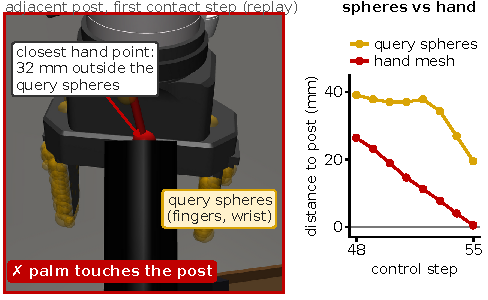
\includegraphics[width=\columnwidth]{../figures/cvpr_v1/fig07_failure.pdf}
\caption{\textbf{Failure case: coverage, not grounding.} With a post directly beside the target, the palm rests on the post at the first contact (red point) while every constraint sphere stays clear of it; the hand point closest to the post lies \pend{32}\,mm outside the sphere union. The frozen policy alone makes the same contact.}
\label{fig:failure}
\end{figure}

A frozen VLA already says which object it is about to touch and what stage of the task it is in; it does not know where that object's surface ends or which of its own links may enter it. \sys\ keeps these questions apart and answers each with the evidence that can: attention seeds, depth continuity bounds, centered features re-identify, physical feedback authorizes, and link-specific fields carry the answers into constrained execution, without an external segmenter or any change to the policy. We see this separation of evidence as what lets geometric safety layers and learned policies share a scene rather than one overruling the other.

\ifhasverifiedreferences
{\small
\bibliographystyle{ieeenat_fullname}
\bibliography{references}}
\else
\section*{References}
\textit{Verified bibliography pending. No citation entries have been fabricated.}
\fi
\end{document}
